% !TEX root = thesis.tex

%%
%%
%% Theoretical background chapter
%%
%%

%%%%%%%%%%%%%%%%%%%%%%%%%%%%%%%%%%%%%%%%%%%%%%%%%%%%%%%%%%%%%%%%%%%%%%%%%%%%%%
%%
%% Disease incidence
%%
%%%%%%%%%%%%%%%%%%%%%%%%%%%%%%%%%%%%%%%%%%%%%%%%%%%%%%%%%%%%%%%%%%%%%%%%%%%%%%
\section{Disease incidence}
\label{sec:theory:incidence}

The theory described in this section is based on \citet{rothman2008modern}.
We study of chronic diseases in order to better understand the degree to which different groups of people are ``at risk'' of contracting a disease.
We also are interested in discovering and describing the association between environmental factors and this ``risk''.
For example, one could ask if air pollution emitted by a factory is associated with an increased ``risk'' of lung cancer among people that live close by.

In order to be more precise, we begin by defining the \textbf{\gls{risk}}:

\begin{defn}
    The \textbf{\gls{risk}} is the probability of contracting a disease in a specific time period.
\end{defn}

One way to estimate the \gls{risk}, is to look at the historical frequency of contracting of the disease.
The type of study we are interested in involves incidents of a chronic disease.
Therefore, we separately consider those people who contracted the disease under study.
In particular, we are interested in people who did not have the disease at the beginning of the study,
but developed the disease within the study period.
These are new cases of the disease, which we call \textbf{\glspl{incident}}.

\begin{defn}
    An \textbf{\gls{incident}} is a new case of the disease during the study period.
\end{defn}

The common measure of frequency used in the literature compares the number of new cases of a disease to the total exposure time of the population is called the \gls{incidence rate}.

\begin{equation}
    \mbox{\Gls{incidence rate} (common definition)} = \frac{\mbox{number of new cases}}
                                {\displaystyle\smashoperator{\sum\limits_{\mbox{persons}}}\mbox{time spent by person in population}}
\end{equation}

For our simulation study, we can simplify our definition of \gls{incidence rate} by assuming that each person in the population is exposed for the entire study period,
which for simplicity we can set to one (1).
Our simplified definition of incidence rate is then:

\begin{defn}
    The \textbf{\gls{incidence rate}} is the number of new cases in the study period divided by the total population.
    \begin{equation}
        \label{eq:incidencerate}
        \mbox{\Gls{incidence rate}} = \frac{\mbox{number of new cases in a time period}}
                                        {\mbox{number of persons}}
    \end{equation}
\end{defn}

\Glspl{incidence rate} are always expressed in cases per person-time units.
For example, 10 cases of asthma per 100,000 people per year is a valid \gls{incidence rate}.

For a given population, time period, and set of \glspl{incident},
we can compute the overall \gls{incidence rate} by taking the total number of \glspl{incident} and dividing by the total population.
However, we may wish to compare the \gls{incidence rate} at different locations within an area.
To do this, we need to look at the number of cases and the population in the areas that are close to these locations.
If we take can make these areas infinitesimally small,
then we could compute the \gls{incidence rate} point-wise.

\begin{defn}
    \label{defn:incidence_rate}
    The \textbf{point-wise \gls{incidence rate}} is a function that computes the local \gls{incidence rate} at a point by dividing the point-wise value of the number of new cases by the point-wise value of the population.
\end{defn}

From this point onwards, the term \gls{incidence rate} refers to the point-wise \gls{incidence rate}.

%%%%%%%%%%%%%%%%%%%%%%%%%%%%%%%%%%%%%%%%%%%%%%%%%%%%%%%%%%%%%%%%%%%%%%%%%%%%%%
%%
%% Spatial point processes
%%
%%%%%%%%%%%%%%%%%%%%%%%%%%%%%%%%%%%%%%%%%%%%%%%%%%%%%%%%%%%%%%%%%%%%%%%%%%%%%%
\section{Spatial point processes}
\label{sec:theory:spatial_point_processes}

The theoretical results in this section are taken from \citet{diggle1983spatial},
\citet{diggle1988equivalence},
\citet{guan2008consistent},
\citet{silverman1986density},
and \citet{wand1994kernel}.

In order to understand the geospatial patterns of disease incidence,
we consider points in two-dimensional space $\RS$.
We begin by defining

\begin{defn}
    A \textbf{study area} $\gls{W} \subset \RS$ is a region in the plane where we make observations.
\end{defn}

The observations we are interested in are points distributed in \gls{W} which we call \textbf{events}.

\begin{defn}
    \label{defn:event}
    An \textbf{event} is a point $\xvec \in \RS$, situated in a study area \gls{W} that we are interested in observing.
\end{defn}

For example, in the study area of the boundaries of a city, we consider the events of the addresses of the residents.
We call this set of events

\begin{defn}
    The \textbf{population} \gls{P} is the set of home address events of the residents of the study area \gls{W}.
\end{defn}

In general, we are interested in the understanding the mechanism by which the events occurred.
We are interested both in the number of events, and even more so in the pattern by which their locations are distributed in \gls{W}.
Taking a spatial statistical approach, we model the underlying mechanism that generates events using the following:

\begin{defn}
    A \textbf{\gls{spp}} $\boldsymbol{\gls{Lambda}}$ is a stochastic mechanism which generates a random set of events.
\end{defn}

Suppose we have a \gls{spp} \gls{Lambda} on a study area $\gls{W} \subset \RS$.
We can count the total number of \glspl{event} and divide it by the total area of \gls{W}.
This gives us a quantity we call the \textbf{average \gls{intensity}} of \gls{Lambda}.
Sometimes the points are spread uniformly throughout \gls{W}.
In that case, we say that \gls{Lambda} is a homogeneous point process.
On the other hand, it is often the case that \gls{Lambda} is not uniform,
and we call it a heterogeneous point process.
When \gls{Lambda} is heterogeneous,
we would like to know the average \gls{intensity} around different points in \gls{W}.
For this, we define $\ds$ as an infinitesimal area around the point $\xvec$,
and the \textbf{\gls{intensity}} $\boldsymbol{\gls{lambda}\xvec}$ at $\xvec \in RS$ as:

\begin{equation}
    \label{eq:lambda_differential}
    \lambda \xvec = \lim_{|\ds| \to 0}
        \left\{
            \frac{\mathbb{E}[N(\ds)]}% /
            {|\ds|}
        \right\}
\end{equation}

And $\gls{lambda}\xvec \ds$ is the approximate probability of \ds~ containing a single incident.
Qualitatively, an intensity function differs from a probability density function in that it does not necessarily integrate to $1$.
In particular, we can write $\gls{lambda}$ as a scaled probability density function
where $f$ is a probability density function and \gls{mu} is a constant.

\begin{equation}
    \label{eq:lambda_mu}
    \gls{lambda}\xvec = \mu f\!\xvec
\end{equation}

For a point-wise \gls{incidence rate} function,
we can compute two separate \gls{intensity} functions.
The first \gls{intensity} returns the point-wise expected number of cases of the disease,
while the second returns the point-wise population density.
Dividing the value obtained from first by the value obtained from the second results in the \gls{incidence rate} described in \Cref{defn:incidence_rate}.

%%%%%%%%%%%%%%%%%%%%%%%%%%%%%%%%%%%%%%%%%%%%%%%%%%%%%%%%%%%%%%%%%%%%%%%%%%%%%%
%%
%% Kernel estimation of the intensity
%%
% %%%%%%%%%%%%%%%%%%%%%%%%%%%%%%%%%%%%%%%%%%%%%%%%%%%%%%%%%%%%%%%%%%%%%%%%%%%%%%
\section{Kernel estimation of the intensity}
\label{sec:theory:kernelestimation}

This section is based on \citet{silverman1986density} and \citet{wand1994kernel}.
The usual case in practice is to start with a set of \glspl{event} that have been observed in a study area.
For example, we can have new cases of a disease in a city that were diagnosed over the course of a defined time period.
By our \Cref{defn:event},
we consider the location coordinates such as those of the home addresses of the people who were diagnosed.
Our goal is to estimate the \gls{intensity} function for disease cases using these observed \glspl{event}.
Similarly for the population,
we would like to estimate the population \gls{intensity} function.

A common method for estimating \gls{intensity} functions is known as
\textbf{\gls{kernel intensity estimator}}.
This technique utilizes a special function known as a \textbf{\gls{kernel}},
denoted by $\gls{K}\xvec$,
that satisfies

\begin{align}
    \gls{K}\xvec \ge 0~ \forall \xvec \in W, \text{and} \label{eq:k_pos} \\
    \iintW{\gls{K}\xvec} & = 1 \label{eq:k_1} \text{.}
\end{align}

\Cref{eq:k_pos,eq:k_1} are equivalent to stating that \Kdots is a probability density on $\RS$.
Starting with a set of \glspl{event} $\gls{N} \subset \RS$,
and a positive value \gls{h} known as the bandwidth,
we define the the \gls{kernel intensity estimator} as follows:

\begin{defn}
    \label{defn:lambda_hat}
    The \textbf{\gls{kernel intensity estimator}} $\gls{lambda_hat}(\xvec;h)$
    is a technique for estimating the \gls{intensity} of an \gls{spp}
    from observed \glspl{event} \gls{N}.
    The formula for computing the \gls{kernel intensity estimator} is:
    \begin{equation}
        \label{eq:lambda_hat}
        \gls{lambda_hat}(\xvec; h) 
            = \sumS{\gls{K}\left(\frac{\xvec-(s_1, s_2)}{h^2}\right)} \text{.}%
    \end{equation}
\end{defn}

This is a natural extension to $\RS$ of the one dimensional \gls{kernel intensity estimator} $\gls{lambda_hat}_1(x;h)$,
which has the formula

\begin{equation}
    \label{eq:lambda_hat_1}
    \gls{lambda_hat}_1(x;h) = \sumSone{K_1\left(\frac{x - s}{h}\right)} \text{.}%
\end{equation}

Here, $K_1(x)$ is a one-dimensional kernel function.

In order to compute \gls{lambda_hat} using \Cref{eq:lambda_hat},
there are two choices to be made: the choice of the bandwidth \gls{h}
and the choice of \gls{kernel} \gls{K}.
The role of the \gls{kernel} function \Kdots is to smooth the information obtained
from the observed \glspl{event} to an area around their locations.
Choosing different \glspl{kernel} results in different shapes to this smoothing.
However, this has only a small effect on the resulting \gls{intensity} estimate.
On the other hand,
the choice of bandwidth \gls{h} has a major effect on the \gls{intensity} estimate.
The bandwidth controls the width of the area smoothed by the \gls{kernel} function and hence on the overall amount of smoothing.

\Cref{fig:theory:kernel1d} shows an example of how \gls{kernel} smoothing works in  one-dimension for three different bandwidths.
The two-dimensional case is analogous.
The dots along the bottom are the observed \glspl{event}.
The dashed lines show the \gls{kernel} functions around each of these \glspl{event},
while the upper solid line is the \gls{intensity} estimate produced using \Cref{eq:lambda_hat_1}.
\Cref{fig:theory:kernel1d:02} shows the estimate with $h=0.2$.
It has two local modes, each with a bit of fluctuation at the peaks.
In \Cref{fig:theory:kernel1d:04} we still see two modes with $h=0.4$, but with smoother peaks.
\Cref{fig:theory:kernel1d:08} has smoothed the two peaks together into a single,
large peak by using the larger bandwidth of $h=0.8$.

\begin{figure}[htbp]
    \centering
    \begin{subfigure}[t]{0.32\textwidth}
        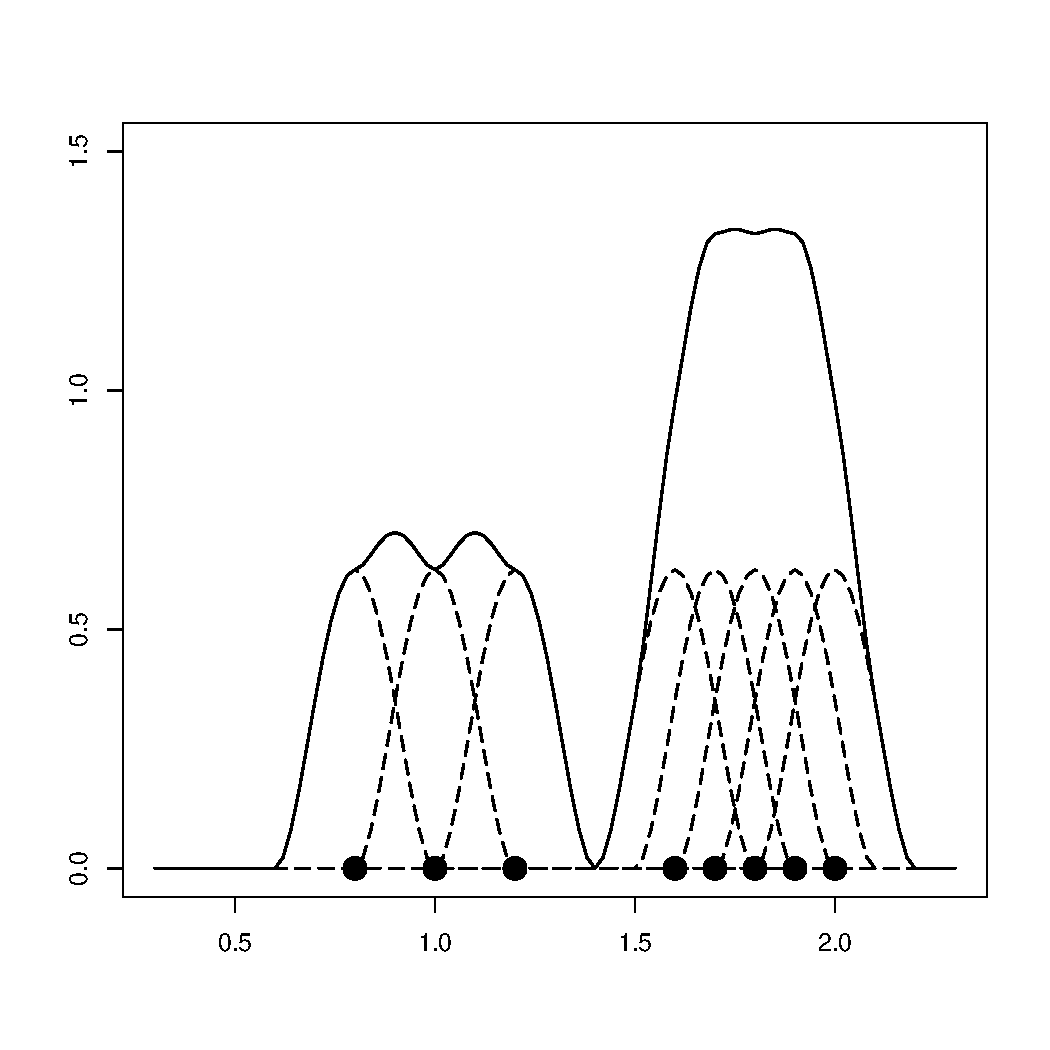
\includegraphics[width=\textwidth]{img/kernel1d-02}
        \subcaption{$h=0.2$}
        \label{fig:theory:kernel1d:02}
    \end{subfigure}
    \begin{subfigure}[t]{0.32\textwidth}
        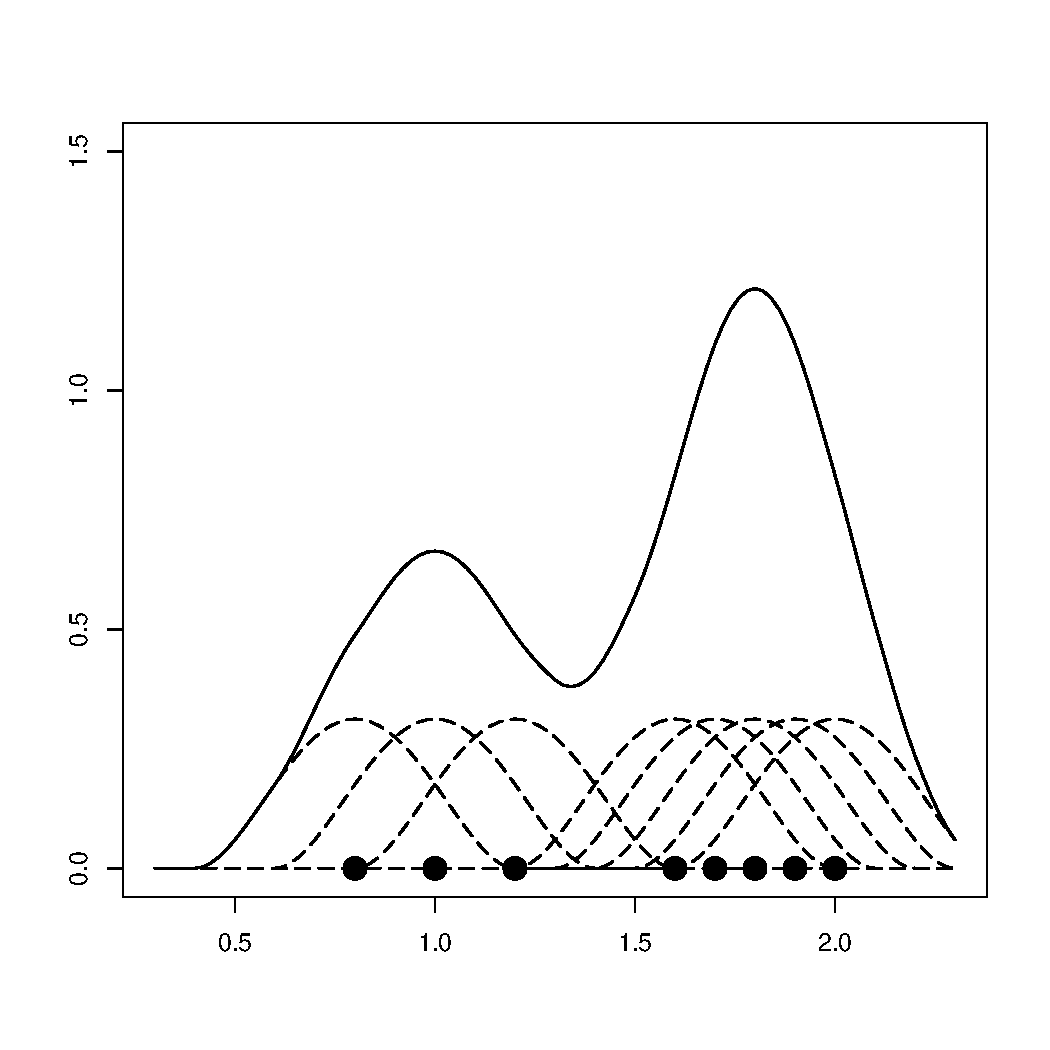
\includegraphics[width=\textwidth]{img/kernel1d-04}
        \subcaption{$h=0.4$}
        \label{fig:theory:kernel1d:04}
    \end{subfigure}
    \begin{subfigure}[t]{0.32\textwidth}
        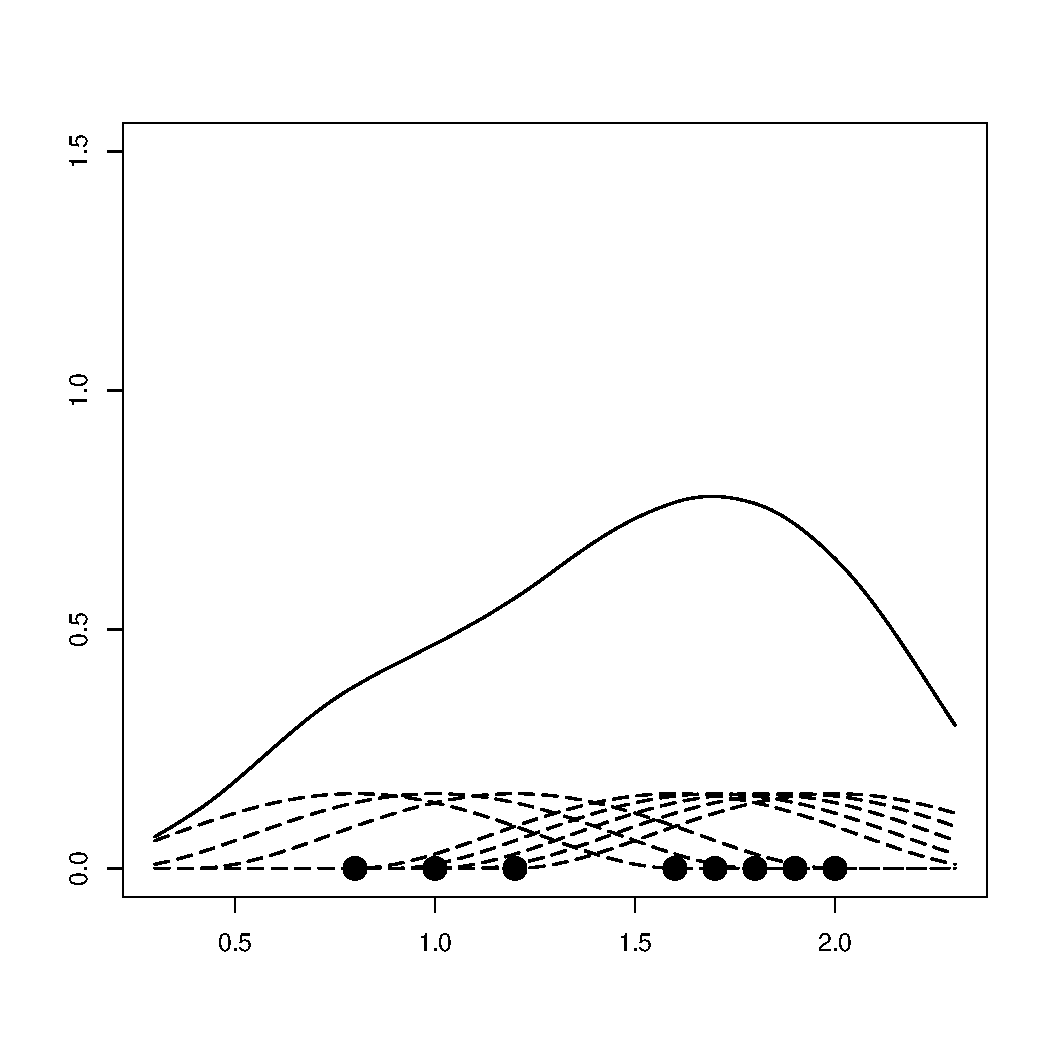
\includegraphics[width=\textwidth]{img/kernel1d-08}
        \subcaption{$h=0.8$}
        \label{fig:theory:kernel1d:08}
    \end{subfigure}
    \caption{One-dimensional \glsentryname{kernel} functions. The dots on the $x1$ axis are the observed \glsentryplural{event}. The dashed lines are the kernel functions around these \glsentryplural{event} and the solid line is the \glsentryname{intensity} estimate $\hat{\lambda_1}$.}
    \label{fig:theory:kernel1d}
\end{figure}

%%%%%%%%%%%%%%%%%%%%%%%%%%%%%%%%%%%%%%%%%%%%%%%%%%%%%%%%%%%%%%%%%%%%%%%%%%%%%%
%%
%% Bandwidth selection
%%
% %%%%%%%%%%%%%%%%%%%%%%%%%%%%%%%%%%%%%%%%%%%%%%%%%%%%%%%%%%%%%%%%%%%%%%%%%%%%%%
\section{Bandwidth selection}
\label{sec:theory:bandwidth}

This section is based on \citet{silverman1986density} and \citet{wand1994kernel}.
A common statistical problem is to find the ``best'' estimate \gls{lambda_hat}
for the \gls{intensity} of an unknown \gls{spp}
based on a set of observed \glspl{event}.
In order to do this using \gls{kernel intensity estimator},
we must select the ``best'' bandwidth.
From \Cref{fig:theory:kernel1d} we can see that different values of bandwidth \gls{h} result in different estimates for the \gls{intensity}.
Our goal is to find a decision procedure that gives us the ``best'' result.

The first thing we must do is define what we mean by the ``best'' result.
We do this by choosing a measure of accuracy for the estimate,
and selecting the bandwidth which gives the optimal value for this measure.
One common accuracy measure used for function estimation is the \gls{mise},
because it has several useful mathematical properties.
It allows for additional analysis by being broken down into the mean integrated squared bias and mean integrated variance.
It can also be easily approximated by cross-validation error.

Given a realized estimate \gls{lambda_hat} for any function \gls{lambda},
we can compute the squared error at any given point $\xvec \in \RS$ as
$\left( \hat{\lambda}\xvec - \lambda\xvec \right)^2$,
and its expected value at $\xvec$ is called the \gls{mse}.
However,
we would like to compute the accuracy of the whole function.
We do this by integrating the squared error of the estimate over the study area to obtain the \gls{ise}.

\begin{equation}
\label{eq:ise}
    \mbox{ISE}(\hat{\lambda}) = \iintW{
            \left( \hat{\lambda}\xvec - \lambda\xvec \right)^2
        }
\end{equation}

The \gls{mise} is the expected value of the \gls{ise} over the sample space of realizations of \gls{Lambda}.

\begin{align}
    \mbox{MISE}(\gls{lambda_hat}) & = \E [\mbox{ISE}(\hat{\lambda})] \nonumber \\
                & = \E \iintW{ \left( \hat{\lambda}\xvec - \lambda\xvec \right)^2 } \label{eq:mise}
\end{align}

The integrand of \Cref{eq:mise} is non-negative.
Therefore, by Fubini's Theorem, we can change the order of integration and expectation.

\begin{align}
    \mbox{MISE}(\gls{lambda_hat}) & = \iintW{ \E \left( \hat{\lambda}\xvec - \lambda\xvec \right)^2 } \nonumber \\
                & = \iintW{ \E \left( \hat{\lambda}\xvec - \E \hat{\lambda}\xvec + \E \hat{\lambda}\xvec - \lambda\xvec \right)^2 } \nonumber \\
                & = \iintW{ \E \left( \hat{\lambda}\xvec - \E \hat{\lambda}\xvec \right)^2 } \nonumber \\
                    & \qquad + 2 \iintW{
                    \E \left\{
                        \left( \hat{\lambda}\xvec - \E \hat{\lambda}\xvec \right)
                        \left( \E \hat{\lambda}\xvec - \lambda\xvec \right)
                    \right\} } \nonumber \\
                    & \qquad + \iintW{ \E \left( \E \hat{\lambda}\xvec - \lambda\xvec \right)^2 } \label{eq:mise_expanded}
\end{align}

The second term of \Cref{eq:mise_expanded} evaluates to zero,
because $\E \hat{\lambda}\xvec$ and $\lambda\xvec$ are numbers,
so
$$\E \left\{
    \left( \hat{\lambda}\xvec - \E \hat{\lambda}\xvec \right)
    \left( \E \hat{\lambda}\xvec - \lambda\xvec \right)
\right\}
$$
is equivalent to
$$ 
\left( \E \hat{\lambda}\xvec - \E \hat{\lambda}\xvec \right)
\left( \E \hat{\lambda}\xvec - \lambda\xvec \right) \text{,}
$$
a product whose first term is zero.
We then have 

\begin{align}
    \mbox{MISE}(\gls{lambda_hat}) & = \iintW{
        \E \left( \gls{lambda_hat}\xvec - \E \hat{\lambda}\xvec \right)^2 } \nonumber \\%
                                  & \qquad %
        + \iintW{ \E \left( \E \gls{lambda_hat}\xvec - \lambda\xvec \right)^2 } \label{eq:mise_bias_variance}%
\end{align}

which is the integrated variance of \gls{lambda_hat} and the integrated squared bias of \gls{lambda_hat}.

%%%%%%%%%%%%%%%%%%%%%%%%%%%%%%%%%%%%%%%%%%%%%%%%%%%%%%%%%%%%%%%%%%%%%%%%%%%%%%
%%
%% Bias and variance
%%
%%%%%%%%%%%%%%%%%%%%%%%%%%%%%%%%%%%%%%%%%%%%%%%%%%%%%%%%%%%%%%%%%%%%%%%%%%%%%%
\section{Bias and variance of kernel intensity estimator}
\label{sec:theory:bias_variance}


The bias of any estimate \gls{lambda_hat} is:

\begin{equation}
    \mbox{bias}(\gls{lambda_hat}) = \E \gls{lambda_hat}\xvec - \gls{lambda}\xvec%
\end{equation}

For the \gls{kernel intensity estimator}, the bias depends on the bandwidth.

\begin{equation}
    \mbox{bias}_h(\gls{lambda_hat}) = \E \left\{%
            \sumS{\gls{K}\left(\frac{\xvec-(s_1, s_2)}{h^2}\right)}%
        \right\}%
        - \gls{lambda}\xvec%
\end{equation}

If we let $\gls{lambda} = \gls{mu} f$ where $f$ is a probability density, then at a point $\xvec \in \RS$,
\begin{align}
    \mbox{bias}(\gls{lambda_hat}(\xvec;h)) & \approx
        \frac{1}{2} \mu h^2 ~ \gls{grad}^2\!\left[ f\xvec \right]
            \int { z^2 K(z_1, z_2) \diff{z_1} \diff{z_2)} } \\
    \mbox{var}(\gls{lambda_hat}(\xvec;h)) & \approx
        h^{-2} \mu
            \int { K(z_1, z_2)^2\diff{z_1} \diff{z_2} } f\xvec
\end{align}

Taking derivative by $h$ and setting to $0$, we get that $h_{\mbox{opt}}$ is $O(\mu^{-1/6})$.

Also, as $\mu \to \infty$, both the bias and variance also $\to \infty$,
but the \textit{relative} MISE, taken by dividing by $\mu^2$ results in the relative bias being $O(\mu^{-1/3})$
but the relative variance being $O(\mu^{1/3})$.

%%%%%%%%%%%%%%%%%%%%%%%%%%%%%%%%%%%%%%%%%%%%%%%%%%%%%%%%%%%%%%%%%%%%%%%%%%%%%%
%%
%% Asymptotic behavior of the bandwidth
%%
%%%%%%%%%%%%%%%%%%%%%%%%%%%%%%%%%%%%%%%%%%%%%%%%%%%%%%%%%%%%%%%%%%%%%%%%%%%%%%
\section{Asymptotic behavior of the bandwidth}
\label{sec:theory:asymptotic_bandwidth}

\Gls{silverman}'s Rule of Thumb for selecting bandwidth in $\RS$:

\begin{equation}
\label{eq:silverman}
    h_S = 2.04 * \sigma * n^{-1/6}
\end{equation}

Where $n$ is the observed number of incidents,
$\sigma$ the arithmetic mean of the standard deviations in the $x_1$ and $x_2$ directions.



%%%%%%%%%%%%%%%%%%%%%%%%%%%%%%%%%%%%%%%%%%%%%%%%%%%%%%%%%%%%%%%%%%%%%%%%%%%%%%
%%
%% Inconsistency of the kernel intensity estimator
%%
%%%%%%%%%%%%%%%%%%%%%%%%%%%%%%%%%%%%%%%%%%%%%%%%%%%%%%%%%%%%%%%%%%%%%%%%%%%%%%
\section{Inconsistency of the kernel intensity estimator}
\label{sec:theory:inconsistency}

From \citet{guan2008consistent}:

{
\color{red}
\textbf{The kernel intensity estimator is not consistent.}
This is because, although the kernel only uses local information around the point of interest to compute the estimate.
The resulting estimate has bias that tends to zero.
However it's variance does not diminish because the number of events in any fixed region is of order 1.
}

The paper develops a \textit{new nonparametric intensity estimator} that is consistent under ``some suitable yet reasonable conditions.''

%%%%%%%%%%%%%%%%%%%%%%%%%%%%%%%%%%%%%%%%%%%%%%%%%%%%%%%%%%%%%%%%%%%%%%%%%%%%%%
%%
%% Estimation of the mode
%%
%%%%%%%%%%%%%%%%%%%%%%%%%%%%%%%%%%%%%%%%%%%%%%%%%%%%%%%%%%%%%%%%%%%%%%%%%%%%%%
\section{Estimation of the mode}
\label{sec:theory:mode}

From \citet{bickel2006fast} and \citet{hedges2003comparison}.


%%%%%%%%%%%%%%%%%%%%%%%%%%%%%%%%%%%%%%%%%%%%%%%%%%%%%%%%%%%%%%%%%%%%%%%%%%%%%%
%%
%% Data generation process
%%
%%%%%%%%%%%%%%%%%%%%%%%%%%%%%%%%%%%%%%%%%%%%%%%%%%%%%%%%%%%%%%%%%%%%%%%%%%%%%%
\section{Data generation process}
\label{sec:theory:data}

We generate data for each experiment as follows.
Before we begin, we set the random number seed to a fixed value for all experiments.
The first step is to generate a population.
We choose a distribution function $f_p$ over \gls{W}, and scale it to obtain an the population intensity function \gls{lambda_p} of a \gls{spp} \gls{Lambda} with an expected number of points the same as our chosen population size.
This means that the actual population size may not be exactly what we have chosen.
We then generate points $\xvec$ uniformly in \gls{W} and keep them with probability \gls{lambda_p}$\xvec$.
This gives us our population \gls{P} which use throughout the experiment.
In this way,
if \gls{lambda_p}$\xvec$ has twice the value of \gls{lambda_p}$(y_1, y_2)$ for two points $\xvec$ and $(y_1, y_2)$ in \gls{W},
then we expect to see about twice as many points around $\xvec$ than around $(y_1, y_2)$ in \gls{P}.

Once we have a fixed population, we have need to decide which members of the population constitute the incidents.
The process to generate the incidents is similar to that of the population.
We create an incident intensity function \gls{lambda_i} of a \gls{spp} for incidents.
We then take the points $\xvec \in \gls{P}$ and keep each one with probability \gls{lambda_i}$\xvec$.
This gives us our set of incidents \gls{I}.
Once again, when \gls{I}$\xvec$ is higher than \gls{I}$(y_1, y_2)$,
then the probability of $\xvec \in \gls{I}$ is correspondingly higher than that of $(y_1, y_2)$.